\section{Method 30\%}
Our method is composed of two consecutive operations: detection and classification. For the first one we adopted YOLO, an one-stage detector based on CNNs able to predict bounding boxes from input images directly without a region proposal step, achieving time efficiency and high inference speed. Therefore, it can be used not only for image detection but also for real-time devices. For the latter we built a multi-class classifier which receives as input the object detected. The reason why we don't adopt YOLO for the whole process is linked to the fact that there is a large number of classes to which a traffic sign could belong. Build a network capable of execute both detection and recognition requires a very long training time and one or more accurate and deep datasets.\\ 
One significant aspect that contributed to the choice of YOLO is the fact that it is a young framework constantly updated and supported by its team. In fact, the version used for this project is YOLOv3 \cite{yolov3}, released in 2018. The latest version, YOLOv4 \cite{yolov4}, was published on April 2020 but the lack of papers and projects to compare our results with lead us to choose the v3. 

\subsection{Network setup}
To perform detection we setup the YOLO network in order to make it works with traffic signs.
\begin{figure}[h]
	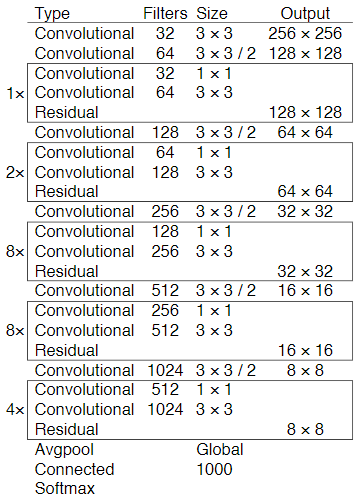
\includegraphics[scale=0.8]{Res/Immagini/darknet53.PNG}	
	\caption{Yolov3 structure called Darknet-53}
\end{figure}

\subsection{YOLO architecture}
\begin{figure}[h]
	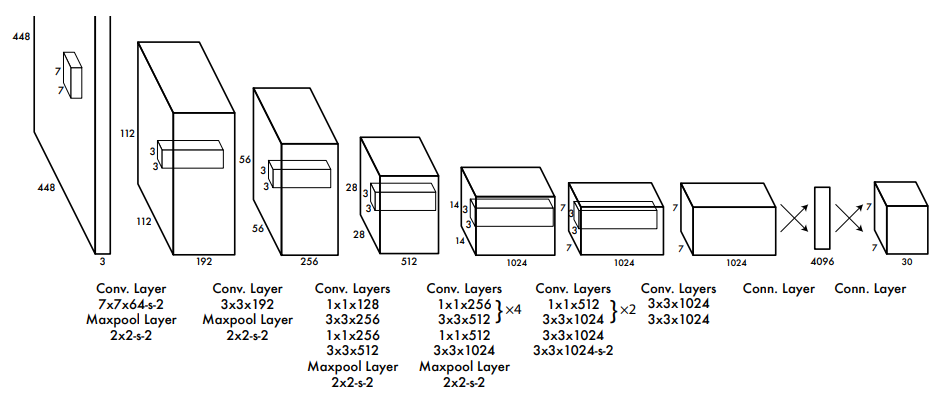
\includegraphics[width=\linewidth]{Res/Immagini/yoloArch.PNG}	
	\caption{YOLO architecture}
\end{figure}
%------------------------------------------------------------------------